\documentclass{article}
\usepackage[utf8]{inputenc}
\usepackage{graphicx}
\graphicspath{ {./images/} }
\usepackage[margin=0.5in]{geometry}
\usepackage{listings}

\title{CSCE  313 Programming Assignment 1}
\author{Hunter Cleary - hncleary - 625001547}
\date{January 2019}

\begin{document}

\maketitle
% \section{}


\section{Buddy Allocator}
\paragraph{} 
\begin{large}
Run-time in microseconds was recorded for both the original code and the completed project. Conditions were set for each possibility within $ 1 < n < 3$ and $ 1 < m < 8 $. 
\end{large}
% Table generated by Excel2LaTeX from sheet 'Sheet1'
\begin{table}[htbp]
  \centering
  \caption{Original Code Run Time}
    \begin{tabular}{rrrrrrrrr}
          & \multicolumn{1}{l}{m} &       &       &       &       &       &       &  \\
    \multicolumn{1}{l}{n} & 1     & 2     & 3     & 4     & 5     & 6     & 7     & 8 \\
    1     & 14    & 143   & 394   & 1329  & 1369  & 1236  & 2372  & 2697 \\
    2     & 304   & 1262  & 2507  & 8965  & 5163  & 7936  & 15865 & 12363 \\
    3     & 8524  & 55711 & 192057 & 767431 & 2987555 & 12168757 & 49822571 & 194735448 \\
    \end{tabular}%
  \label{tab:addlabel}%
\end{table}%
% Table generated by Excel2LaTeX from sheet 'Sheet1'
\begin{table}[htbp]
  \centering
  \caption{Project Code Run-time}
    \begin{tabular}{rrrrrrrrr}
          & \multicolumn{1}{l}{m} &       &       &       &       &       &       &  \\
    \multicolumn{1}{l}{n} & 1     & 2     & 3     & 4     & 5     & 6     & 7     & 8 \\
    1     & 35    & 132   & 405   & 408   & 1228  & 999   & 272   & 616 \\
    2     & 722   & 1246  & 1466  & 2656  & 2257  & 2095  & 2484  & 3044 \\
    3     & 2241  & 2258  & 1730  & 1352  & 7610  & 5970  & 13735 & 23286 \\
          &       &       &       &       &       &       &       &  \\
    \end{tabular}%
  \label{tab:addlabel}%
\end{table}%

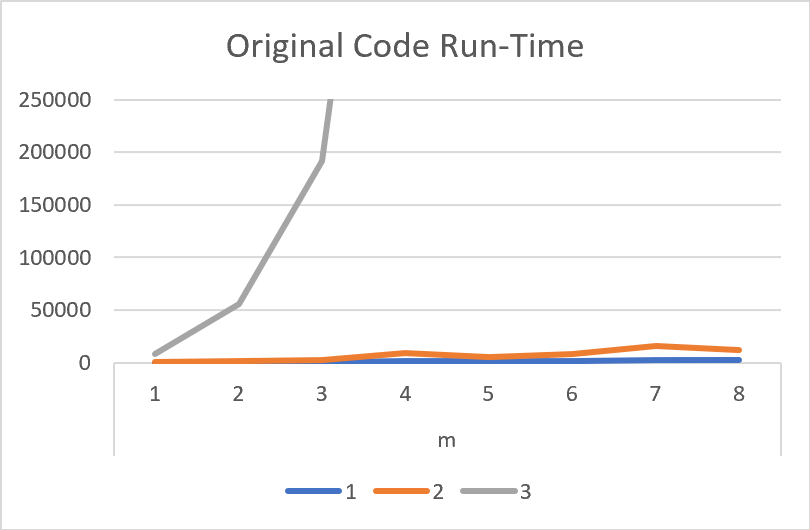
\includegraphics[height=5.3cm ]{Graph2.png}
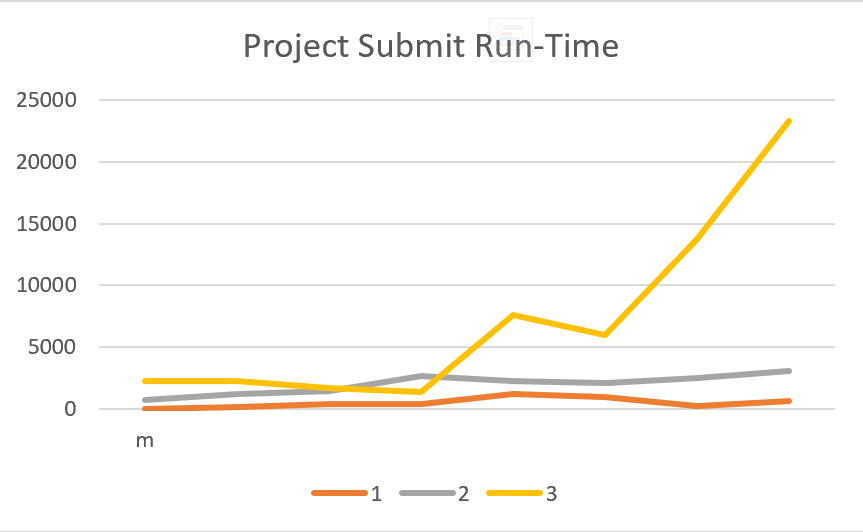
\includegraphics[height=5.3cm ]{graph1.png}

\paragraph{}
\begin{large} There was a clear and significant improvement in run-time when the code was changed. As demonstrated in the graphs and data above, the scale of time taken decreased drastically when the buddy allocator was more properly implemented with an efficient linked list. As allocate and free calls increased, generally, so did the time taken to run. This was especially so when n was $\geq 3$. The run-time increased exponentially in both testing cases, but significantly less so in the improved version, demonstrating that the number of $alloc()$ calls could more drastically change the run-time value.
\\ \\
\ \ \ \ The implementation of the BlockHeader linked list lead to an improved run-time. This allowed the allocator to insert, remove, merge, and split blocks without having to iterate through the entire linked list. Using block member variables, nodes could be found during recursion, allowing functions to be run effectively.



\end{large}

  



\end{document}
